\chapter{Background}
\label{ch2}


\section{Review of Literature}

Diffusion probabilistic models have emerged as a powerful class of generative models that have significantly advanced the field of image generation. These models operate by gradually transforming a distribution of random noise into a distribution of structured images over many iterative steps, effectively reversing the diffusion process. This methodology allows for the generation of highly detailed and coherent images across a range of domains and applications.

One of the most notable achievements of diffusion probabilistic models is their ability to produce images that rival the quality of those generated by other leading techniques, such as Generative Adversarial Networks (GANs). Dhariwal and Nichol report that a diffusion model surpasses the strongest available adversarial baseline on ImageNet synthesis at several resolutions \parencite{arXiv:2105.05233}, and attribute the margin to fidelity and coverage of the data distribution rather than to sample sharpness alone.

In terms of specific accomplishments, diffusion models have excelled in tasks such as high-resolution image synthesis, text-to-image generation, and image-to-image translation. For instance, they have been successfully applied to create photorealistic images of landscapes and portraits from textual descriptions, showcasing their versatility and robustness. Additionally, these models have proven capable of handling complex conditioning information, making them particularly useful for tasks requiring detailed customization of the generated content.

The theoretical underpinnings of diffusion models also contribute to their appeal. Unlike GANs, which can be challenging to train due to issues like mode collapse, diffusion models offer a more stable training process. This stability stems from their foundation in well-understood stochastic differential equations, providing a clear pathway for systematic improvements and adaptations.

\begin{figure}
    \centering
    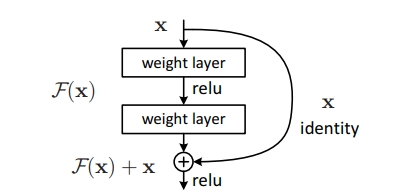
\includegraphics[width=0.5\linewidth]{imgs/Residual_learning.jpeg}
    \caption{Residual Learning: a building block \cite{arXiv:1512.03385}}
    \label{fig:residual-block}
\end{figure}

The ResNet architecture, short for Residual Network, was introduced by He et al.\ in ``Deep Residual Learning for Image Recognition'' \parencite{arXiv:1512.03385} and has since been adopted across a wide range of computer vision tasks.

ResNet’s primary innovation lies in its use of residual blocks (Figure~\ref{fig:residual-block}). These blocks allow the network to skip one or more layers through the use of shortcut connections, or skip connections, that perform identity mapping. By adding the output from an earlier layer to a later layer, these connections help to mitigate the vanishing gradient problem that plagues deep neural networks. As a result, ResNet can effectively train much deeper networks than was previously possible.

The standard implementations of ResNet include variants with different depths, typically ranging from 18 layers to 152 layers. ResNet-50, ResNet-101, and ResNet-152 are among the most popular configurations, with the number indicating the count of layers. These models are established baselines for image classification, detection and segmentation on ImageNet and COCO.

ResNet reduced classification error substantially relative to the plain architectures that preceded it, and ResNet-50 and ResNet-101 in particular are widely used because they balance depth against computational cost.

The architecture has also been applied outside image recognition, including in audio signal processing and reinforcement learning, which indicates that the benefit of residual connections is not specific to the visual domain.

Training diffusion probabilistic models presents a unique set of challenges that are both computational and theoretical in nature. These models operate by learning to reverse a diffusion process, gradually converting random noise into a structured data distribution over many iterative steps. While the results can be impressive, achieving them is far from straightforward.

One of the most significant hurdles in training diffusion models is their high computational cost. Each training iteration involves simulating the reverse diffusion process across multiple timesteps, which can be computationally intensive especially as the number of timesteps increases. This makes training such models resource-heavy, requiring powerful hardware and often resulting in long training times. Researchers have explored methods such as subsampling timesteps during training to reduce computational overhead. This approach is discussed in ``Improved Denoising Diffusion Probabilistic Models'' by Alex Nichol and Prafulla Dhariwal \cite{arXiv:2102.09672}, where they introduce techniques to selectively skip timesteps without compromising the model’s performance. 

The performance of diffusion models heavily relies on the precise tuning of hyperparameters, including the learning rate, the number of diffusion steps, and the noise schedule. Determining the optimal settings for these parameters can be a trial-and-error process that requires extensive experimentation and computational resources.

Although diffusion models are generally more stable during training compared to other generative models like GANs, they are not completely free from stability issues. Problems can arise from numerical instabilities during the simulation of the reverse diffusion process, particularly when dealing with very low probability events in high-dimensional spaces.

Diffusion models are often applied to high-dimensional data such as images, which can complicate the training process. The curse of dimensionality can exacerbate the challenges in modeling the data distribution accurately, requiring more sophisticated techniques and deeper networks. Techniques such as principal component analysis (PCA) and autoencoders have been used to reduce the dimensionality of data before training diffusion models. This can simplify the learning process and improve the manageability of high-dimensional data.

Measuring the performance of diffusion models can also be challenging. Traditional metrics like log-likelihood are not always informative for image quality in visual tasks. Alternatives like Inception Score or Fréchet Inception Distance are commonly used, but they have their limitations and may not fully capture the model’s capabilities in generating diverse and realistic images.

A practical challenge in training diffusion models for image generation is balancing the level of detail in the generated images with the diversity of the output. Overtraining on specific features can lead to loss of diversity (mode collapse), while too much randomness can reduce the realism of the generated images.

Despite these challenges, diffusion models are continuously being refined and improved, making them increasingly viable for a range of applications. Advances in computational resources, algorithmic optimizations, and better understanding of the underlying processes are helping to mitigate these difficulties, broadening the practical use of diffusion models in the field of generative modeling.

Exploring Stochastic Differential Equations (SDEs) as a modeling approach for the diffusion process has become a significant area of research in the development of diffusion probabilistic models. SDEs are used to provide a mathematical framework for modeling the continuous dynamics of the random variables involved in the diffusion process. This approach has several advantages, particularly in terms of flexibility, precision, and the ability to model complex stochastic behaviors.

Stochastic Differential Equations are used to model systems that exhibit random behavior and are influenced by continuous stochastic noise. In the context of diffusion models, SDEs describe how an image (or another data type) gradually transitions from a meaningful configuration to a state of pure noise—and vice versa—over continuous time. This is fundamentally different from the discrete step-wise approach seen in earlier diffusion models, where the process was modeled as a sequence of discrete steps.

In diffusion probabilistic models, the forward process is modeled as adding noise over time until the data becomes indistinguishable from Gaussian noise. The reverse process, which is of primary interest, involves learning the reverse of this noise-adding process. By employing SDEs, researchers can model this reverse process more naturally and fluidly as it provides a continuous-time framework, which can capture the nuances of the noise reduction at any point in time.

SDEs allow the diffusion process to be defined in continuous time, giving a finer control over the dynamics of the process. This can lead to more precise and controlled generation of the data, as the model can potentially make adjustments at any moment in the continuous timeline. The use of SDEs enables the modeling of more complex dynamics that cannot be captured by simple discrete transitions. This is particularly useful in applications where the data exhibits intricate stochastic behaviors. It is also possible to implement more efficient sampling algorithms that leverage the continuous nature of the process. For instance, adaptive step-size solvers can be used to speed up the reverse diffusion process without loss of quality.

\begin{figure}
    \centering
    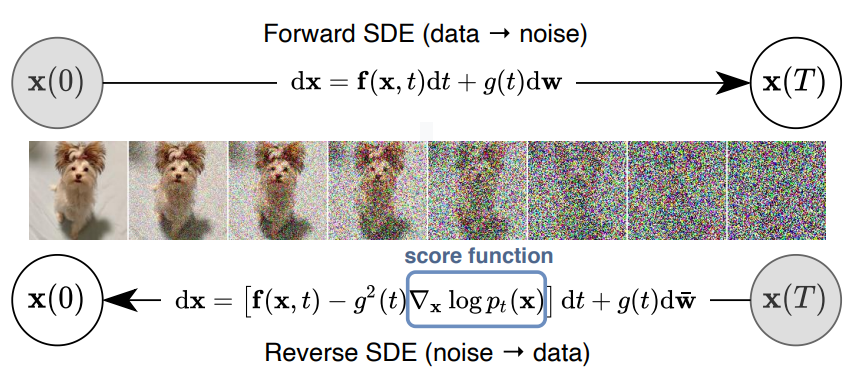
\includegraphics[width=0.5\linewidth]{imgs/Solving_a_reverse-time_SDE.png}
    \caption{Solving a reverse time SDE yields a score-based generative model. Transforming data to a simple noise distribution can be accomplished with a continuous-time SDE. This SDE can be reversed if we know the score of the distribution at each intermediate time step \parencite{arXiv:2011.13456}}
    \label{fig:reverse-sde}
\end{figure}

The seminal work by Yang Song et al. in their paper ``Score-Based Generative Modeling through Stochastic Differential Equations'' published at ICLR 2021 \parencite{arXiv:2011.13456}, is a notable contribution to this area, and the correspondence between the forward and reverse-time processes that it formalises is illustrated in Figure~\ref{fig:reverse-sde}. They propose a framework that uses score-based methods and SDEs to generate samples. By defining the generative model as a solution to an SDE, they are able to leverage the properties of differential equations to model the diffusion process more robustly and efficiently.

Despite the advantages, implementing SDEs in diffusion models also introduces new challenges. The primary issue is the computational cost associated with solving SDEs, especially in high-dimensional spaces typical of image data. Additionally, designing and training models to solve these equations requires sophisticated techniques and a deep understanding of both the theoretical and practical aspects of stochastic calculus.

\section{Analysis of Competing Products}

Denoising Diffusion Probabilistic Models (DDPMs), Variational Autoencoders (VAEs), and Generative Adversarial Networks (GANs) are all prominent types of generative models, each with unique strengths and applications.

\subsection{Variational Autoencoders (VAE)}

Variational Autoencoders (VAEs) have been a significant part of the generative modeling landscape since their introduction by Kingma and Welling in ``Auto-Encoding Variational Bayes'' \parencite{arXiv:1312.6114}. VAEs are especially valued for their robustness in learning latent representations and their ability to generate new data points with variations that are meaningful in a learned latent space.

VAEs are particularly celebrated for their ability to learn well-structured latent spaces. This means that similar data points result in close points in the latent space, making these models excellent for tasks that involve data interpolation, anomaly detection, and more. This has been critical for advancements in fields like bioinformatics where understanding the underlying structure of data is crucial.

Early criticisms of VAEs focused on their tendency to produce blurrier samples compared to GANs. However, advancements have been made to address this issue. Techniques such as using hierarchical latent variables, improving the variational bound, or incorporating better decoder architectures have significantly enhanced the quality of the generated samples. For instance, the introduction of VQ-VAE (Vector Quantized VAE) by van den Oord et al. \parencite{arXiv:1711.00937} and its successor VQ-VAE-2 by Razavi et al. \parencite{arXiv:1906.00446} showcases substantial improvements in the fidelity and diversity of generated images.

VAEs have found applications in a variety of fields beyond just image generation. In drug discovery, VAEs are used to generate novel molecular structures by learning from known chemical compounds. Similarly, in finance, they help in modeling complex financial instruments and in risk management by understanding the distributions of various financial parameters. These applications benefit from VAEs' ability to model complex, high-dimensional data in a compressed, interpretable format.

The flexibility of VAEs allows them to be effectively combined with other neural network architectures, enhancing their utility and performance. For example, the integration of VAEs with Recurrent Neural Networks (RNNs) has led to improved models for sequence data, which is useful in natural language processing and sequential image analysis.

The theoretical aspects of VAEs have also been extensively explored, leading to a deeper understanding and better implementations. Innovations such as the $\beta$-VAE, introduced by Higgins et al. \parencite{higgins2017betavae}, offer a way to balance latent channel capacity and independence constraints to control the disentanglement of latent representations, enhancing both interpretability and control over generative models.

\subsection{Generative Adversarial Networks (GAN)}

Generative Adversarial Networks (GANs) reshaped generative modelling after their introduction by Goodfellow et al.\ \parencite{arXiv:1406.2661}. The unique adversarial training approach of GANs, involving a duel between a generator and a discriminator, has led to substantial advancements in generating high-fidelity and realistic images. The achievements of GANs span various domains, from art creation to medical image analysis. 

The principal achievement of GANs is the visual quality of their samples. BigGAN \parencite{arXiv:1809.11096} and StyleGAN \parencite{arXiv:1812.04948} generate images at resolutions and levels of detail that earlier generative models did not reach, and StyleGAN in particular separates the factors of variation across its layers, so that attributes of the generated image can be controlled independently.

GANs have been successfully applied to a wide range of applications. In the field of fashion, GANs are used for creating new clothing designs and for virtual try-ons. In video games and virtual reality, they help generate realistic environments and characters. Additionally, GANs have made significant impacts in the medical field, where they are used for data augmentation in medical imaging and for generating synthetic patient data that can be used for training other AI models without privacy concerns.

GANs have also been pivotal in advancing unsupervised and semi-supervised learning techniques. The ability of GANs to learn complex distributions without extensive labeled data has made them valuable for scenarios where labeled data is scarce or expensive to obtain. For instance, models like the Semi-Supervised GAN (SGAN) \parencite{arXiv:1606.01583} leverage this capability to improve learning efficiency and accuracy using smaller amounts of labeled data supplemented with larger amounts of unlabeled data.

Despite their potential, GANs were initially known for being difficult to train, with issues such as mode collapse and non-convergence. Over the years, researchers have proposed various techniques to stabilize GAN training, such as introducing new architectures, loss functions, and regularization techniques. The introduction of the Wasserstein GAN (WGAN) \parencite{arXiv:1701.07875} marks a significant development in this area, addressing the issue of training stability through a novel loss function that provides a smoother gradient.

Analysis of the training dynamics, and in particular of how the generator and discriminator interact over the course of optimisation, has informed the architectural and loss-function changes described above.

\section{Specification of Software Standards}

\begin{itemize}
    \item \textbf{Google Python Style Guide} is a comprehensive set of guidelines that Google provides to maintain a consistent and high-quality codebase across its Python projects.
    \item \textbf{NumPy} is a fundamental library for scientific computing in Python, providing support for large, multi-dimensional arrays and matrices, along with a large collection of high-level mathematical functions to operate on these arrays.
    \item \textbf{PyTorch} is an open-source machine learning library developed by Facebook, known for its flexibility and ease of use in building and training deep learning models, particularly popular for research and prototyping.    
\end{itemize}

\section{ResNet Background Theory}

Residual Networks represent a seminal advancement in deep learning that emerged to address the vanishing gradient problem occurring in very deep neural networks. ResNet fundamentally altered approaches to network architecture design, enabling the training of networks that are substantially deeper than those previously feasible. This development has had profound implications for the field of computer vision and beyond. 

Before ResNet, increasing network depth to improve performance had reached a bottleneck. Typically, deeper networks begin to suffer from the vanishing gradient problem—where gradients become too small to make meaningful adjustments in weights during backpropagation—leading to saturation and then rapid degradation of training accuracy. Moreover, deeper networks often encounter a complexity that makes them computationally expensive and harder to optimize.

ResNet introduced a novel solution to these issues through the use of residual learning. The central hypothesis was that if deeper networks are approximations of shallower ones, then it should be easier to optimize the residual mappings rather than the desired underlying mapping.

The core idea behind ResNet is the introduction of the residual block, which includes shortcut connections (also known as skip connections). These connections allow the input to a layer to be added to its output, effectively forming an identity mapping that skips one or more layers. Mathematically, if $H(x)$ is an underlying mapping to be learned by a few stacked layers, and $x$ is the input, then these layers in ResNet fit another mapping of \eqref{eq:residual-function}. The original function thus becomes \eqref{eq:residual-identity}.

\begin{equation}
    F(x) := H(x) - x \label{eq:residual-function}
\end{equation}

\begin{equation}
    H(x) = F(x) + x \label{eq:residual-identity}
\end{equation}

This setup makes it easier to optimize the network because learning the residual mapping $F(x)$ is simpler than learning the unreferenced mapping $H(x)$. In practice, this means that even very deep networks can be trained directly through standard backpropagation. This approach addresses both the degradation problem—ensuring that adding more layers does not lead to higher training error—and reduces the impact of the vanishing gradients by providing an alternative pathway for gradient flow during backpropagation.

\begin{figure}
    \centering
    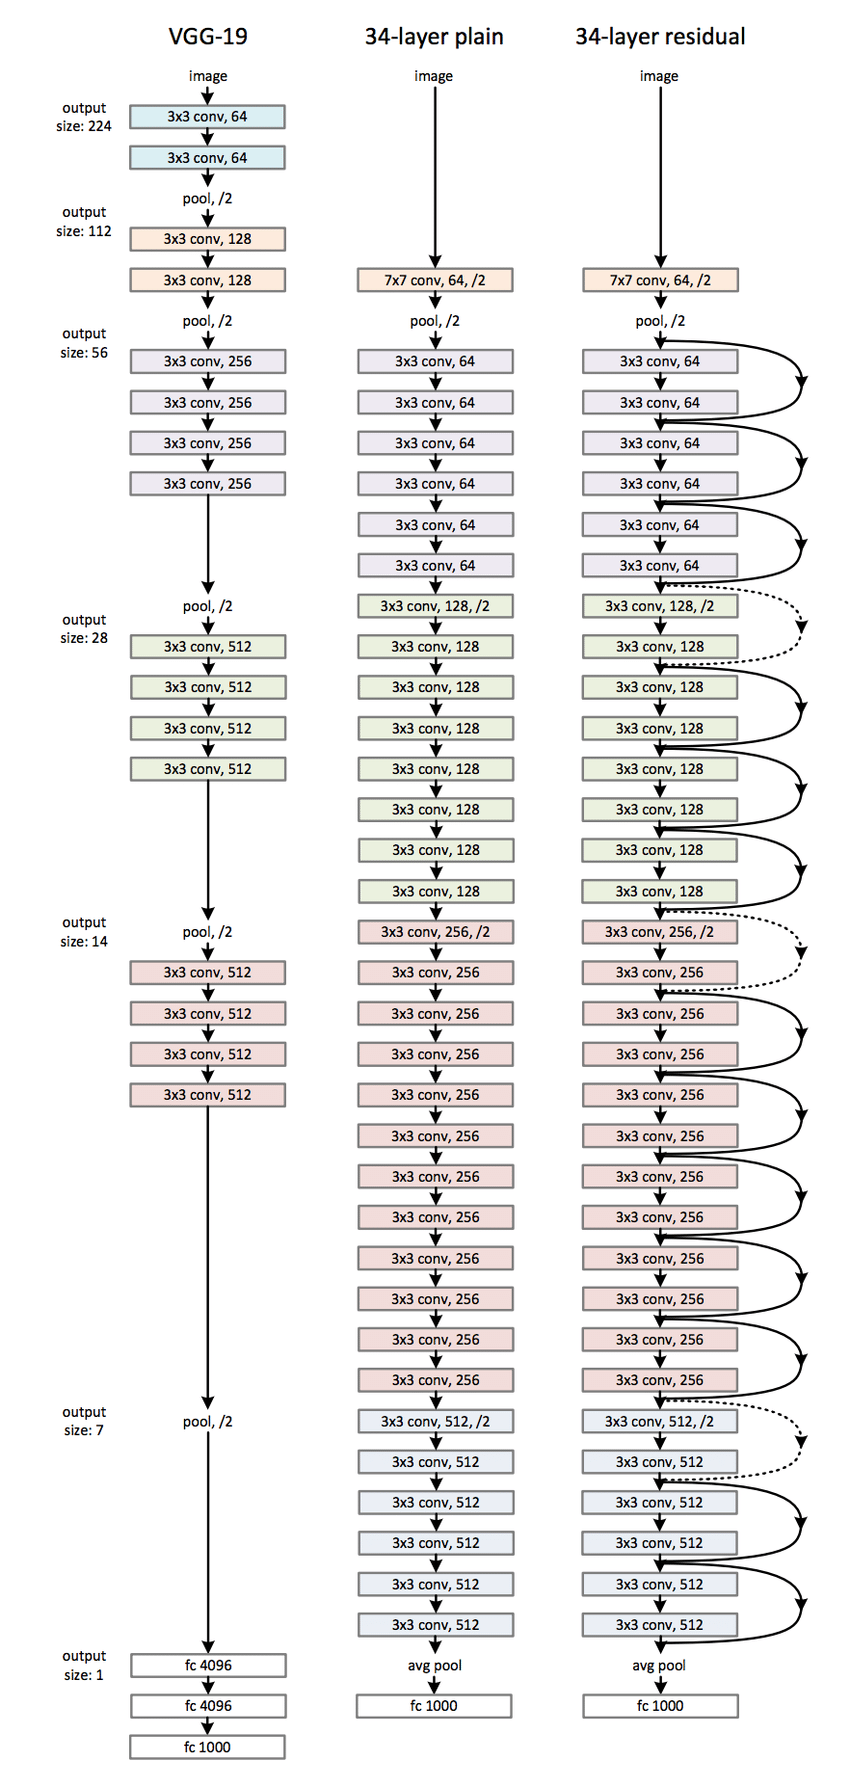
\includegraphics[width=0.5\linewidth]{imgs/Example-network-architectures-for-ImageNet-Left-the-VGG-19-model-196-billion-FLOPs.png}
    \caption{Example network architectures for ImageNet. \textbf{Left}: the VGG-19 model \parencite{arXiv:1409.1556} (19.6 billion FLOPs) as a reference. \textbf{Middle}: a plain network with 34 parameter layers (3.6 billion FLOPs). \textbf{Right}: a residual network with 34 parameter layers (3.6 billion FLOPs). The dotted shortcuts increase dimensions. \parencite{arXiv:1512.03385}}
    \label{fig:resnet-architectures}
\end{figure}

The standard ResNet models are implemented with varying depths, including ResNet-18, ResNet-34, ResNet-50, ResNet-101, and ResNet-152, which indicate the number of layers. Each ResNet block is a composition of several convolutional layers, batch normalization layers, and ReLU activations. In deeper ResNet versions (50, 101, 152), bottleneck layers are introduced to reduce the model size and complexity. Each convolutional layer within these bottlenecks is tightly packed with $1\times 1$ and $3\times 3$ convolutions.

\subsection{Plain Network}

The plain network architecture referenced in the context of ResNet typically comprises stacked convolutional layers, where each layer is followed by batch normalization and a ReLU activation function (Figure~\ref{fig:resnet-architectures}, \textbf{Left}). This architecture builds on the basic principles of CNNs, which are designed to capture hierarchical patterns in image data through a series of filtering and pooling operations. 

In a plain network, convolutional layers form the core components. These layers apply a set of learnable filters to the input image, capturing various features at different levels of abstraction. For example, the initial layers might capture simple features like edges and textures, while deeper layers capture more complex patterns such as object parts.

Following each convolutional operation, batch normalization is applied. This technique normalizes the input layer by adjusting and scaling the activations, helping to maintain mean output close to 0 and the output standard deviation close to 1. This normalization helps to combat issues in training deep networks by stabilizing the learning process and reducing the number of training epochs required.

After batch normalization, a non-linear activation function—typically the Rectified Linear Unit (ReLU)—is used. The ReLU function introduces non-linear properties to the system, allowing the network to learn more complex patterns. It is defined as $f(x)=max(0,x)$, which has been shown to accelerate the convergence of stochastic gradient descent compared to traditional sigmoid or tanh functions.

The architecture often includes pooling layers, which reduce the spatial size of the representation, diminishing the amount of parameters and computation in the network. Pooling helps in making the detection of features invariant to scale and orientation changes.

Towards the end of the network, fully connected layers are typically used to map the learned features to the desired output size. For instance, in classification tasks, these layers might culminate in a softmax activation function that distributes the output into probability scores corresponding to various classes.

The plain architecture, while foundational, encounters significant challenges as network depth increases:

\begin{itemize}
    \item \textbf{Vanishing and Exploding Gradients}: In very deep networks, gradients propagated back through the network can vanish (become very small) or explode (become very large), which significantly hampers the ability to learn.
    \item \textbf{Degradation Problem}: As depth increases, network accuracy gets saturated and then degrades rapidly. Interestingly, this degradation is not due to overfitting, and adding more layers leads to higher training error.
\end{itemize}

The plain network architecture is crucial for understanding the baseline upon which ResNet improves. By addressing the shortcomings of the plain networks, especially the degradation problem through the introduction of skip connections (or shortcut connections), ResNet allows much deeper networks to be trained effectively. This capability to train deeper networks without a drop in performance has set new benchmarks in various machine learning tasks and underscores the transformative impact of ResNet in the landscape of deep learning.

\subsection{Residual Network}

The cornerstone of the ResNet architecture is the concept of residual learning. As networks deepen, training becomes increasingly difficult due to the vanishing gradient problem, where gradients of the network's layers diminish as they propagate back through the network during training. Traditional networks attempt to learn the desired underlying mapping directly. In contrast, ResNet reformulates the layers as learning residual functions with reference to the layer inputs, thereby simplifying the learning process (Figure~\ref{fig:resnet-architectures}, \textbf{Right}).

A typical ResNet is composed of several stacked residual blocks. Each residual block has two main pathways:

\begin{itemize}
    \item \textbf{Identity Shortcut Connection}: This pathway allows the input to bypass the main layers of the block and connect directly to the output of the block, adding the input $x$ to the output of the block's layers $F(x)$. This direct path forwards the input without any alteration, preserving the strength of the gradient as it back-propagates through the network.
    \item \textbf{Weighted Layers}: Typically consisting of two or three convolutional layers (depending on the variant of ResNet), each followed by batch normalization and a ReLU activation function. These layers aim to learn the residual functions, denoted as $F(x)$, where $x$ is the input to the layers.
\end{itemize}

The output of a residual block is then \eqref{eq:residual-identity}, where $F(x)$ represents the learned residual function and $x$ is the identity mapping. The addition of $F(x)$ and $x$ is element-wise and may involve dimensionality adjustments (using $1\times 1$ convolutions) if necessary to match the dimensions.

ResNet comes in various depths, which are generally tailored to the complexity of the tasks they are intended to perform. Common variants include:

\begin{itemize}
    \item \textbf{ResNet-18} and \textbf{ResNet-34}: These versions use blocks with two convolutional layers each.
    \item \textbf{ResNet-50}, \textbf{ResNet-101}, and \textbf{ResNet-152}: These deeper models utilize bottleneck blocks designed to reduce the model size and computational load. A bottleneck block contains three layers: a $1\times 1$ convolution that reduces the dimension, a $3\times 3$ convolution, and another $1\times 1$ convolution that restores the dimension.
\end{itemize}

In this project the denoising network is not one of the standard ImageNet classifiers but a residual UNet (ResUNet) assembled from the basic two-layer residual block described above. Bottleneck blocks of the kind used in ResNet-50 are designed for the deep, heavily downsampled feature hierarchies demanded by $224 \times 224$ ImageNet classification; at the $32 \times 32$ resolution of CIFAR-10 the spatial extent is exhausted after only a few downsampling stages, so the additional $1 \times 1$ compression they provide yields little benefit for a considerable increase in implementation complexity. A shallower network built from basic blocks is therefore adopted, and the classification head is replaced by an encoder-decoder structure so that the network maps an image to an image rather than to a class score, as a denoising network must.

The resulting architecture retains two downsampling stages at the $32 \times 32$ resolution of CIFAR-10. At the $64 \times 64$ resolution of CelebA a third stage is inserted and the channel widths are narrowed accordingly, so that the two configurations remain comparable in size.

\begin{itemize}
    \item \textbf{Encoder stage 1} maps the three input channels to 64 feature channels at $32 \times 32$, after which max pooling halves the resolution.
    \item \textbf{Encoder stage 2} maps 64 channels to 128 at $16 \times 16$, followed by a second max pooling to $8 \times 8$.
    \item A \textbf{residual bridge} operates on the 128 channels at the coarsest resolution.
    \item \textbf{Decoder stage 2} upsamples to $16 \times 16$ by transposed convolution and concatenates the stage-2 encoder features, giving 256 channels.
    \item \textbf{Decoder stage 1} upsamples to $32 \times 32$ and concatenates the stage-1 encoder features, giving 128 channels.
    \item A final $1 \times 1$ convolution projects the 128 channels back to the three image channels.
\end{itemize}

Each residual block follows the two-layer form used in ResNet-18 and ResNet-34: a $3 \times 3$ convolution, a normalisation layer, a non-linear activation, a second $3 \times 3$ convolution and a further normalisation, with the block input added to the result. Group normalisation is used in place of the batch normalisation of the original ResNet. The running statistics that batch normalisation accumulates would be estimated over clean images, whereas the input actually presented to a denoising network is the noised image $x_t$, whose distribution changes with the timestep; group normalisation avoids this mismatch by normalising within each example. Because the channel count is preserved within a block, the shortcut is a pure identity mapping and no $1 \times 1$ projection is required. The connections between corresponding encoder and decoder stages are concatenations rather than additions, which is the convention inherited from the UNet family and is what allows the fine spatial detail lost during downsampling to be recovered in the decoder.

\subsection{Reference Denoising Architecture}

The network proposed above is assessed against the denoising architecture introduced with the DDPM itself \parencite{arXiv:2006.11239}, which serves as the reference design throughout this work. It is also a UNet built from residual blocks, but differs from the network of the previous section in four respects.

\begin{itemize}
    \item It uses \textbf{four resolution stages} rather than two or three, so the coarsest feature map is reached through a deeper hierarchy.
    \item \textbf{Self-attention} is inserted at the $16 \times 16$ resolution and at the bottleneck, giving each spatial position access to the whole feature map rather than only to its convolutional neighbourhood.
    \item A \textbf{skip connection is taken from every residual block}, not one per resolution stage, so the decoder receives a considerably finer record of the encoder activations.
    \item Resolution is changed by \textbf{strided convolution and nearest-neighbour upsampling followed by convolution}, in place of max pooling and transposed convolution.
\end{itemize}

Because the channel count varies within a stage, the shortcut in these blocks cannot be a pure identity mapping and a $1 \times 1$ projection is applied where the dimensions differ. The configuration published for CIFAR-10 uses a base width of 128 channels and amounts to roughly 35 million parameters, which is more than an order of magnitude larger than the network proposed here. Comparing the two at their published sizes would confound architecture with capacity, so the base width is reduced until the parameter counts agree to within a few per cent; the comparison then reflects the arrangement of the layers rather than the number of them.

\section{Diffusion Model Background Theory}

Diffusion models (Figure~\ref{fig:diffusion-overview}) operate by modeling the data generation process as a Markov chain of gradual, stepwise transformations from a data distribution into a predetermined noise distribution, typically Gaussian noise. This process is characterized mathematically by a series of forward diffusion steps that progressively add noise to the data until only noise remains.

\begin{figure}
    \centering
    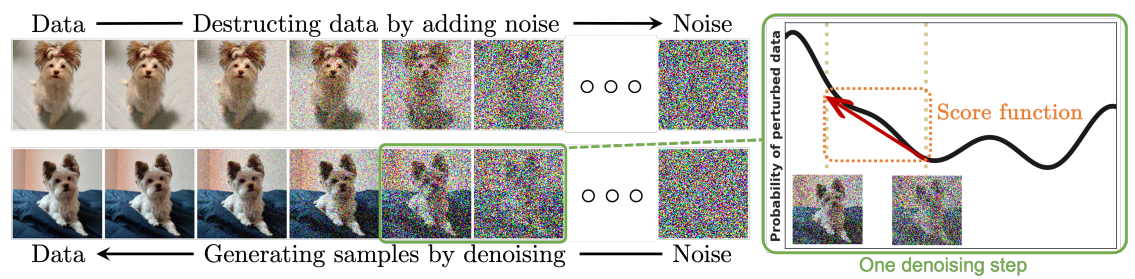
\includegraphics[width=0.5\linewidth]{imgs/Diffusion models.png}
    \caption{ Diffusion models smoothly perturb data by adding noise, then reverse this process to generate new data from noise. Each denoising step in the reverse process typically requires estimating the score function (see the illustrative figure on the right), which is a gradient pointing to the directions of data with higher likelihood and less noise. \parencite{arXiv:2209.00796}}
    \label{fig:diffusion-overview}
\end{figure}

\subsection{Forward Process}

The forward process (or the diffusion process) can be described by the following stochastic differential equation (SDE):

\begin{equation}
    dX_{t} = -\frac{1}{2}\beta(t)X_{t}dt+\sqrt{\beta(t)}dW_t \label{eq:forward-sde}
\end{equation}

Here, $X_t$ represents the data at time $t$, $\beta(t)$ is a variance schedule that governs the noise level at each step, and $dW_t$ denotes the increment of a Wiener process, reflecting the stochastic nature of the noise addition. The parameter $\beta(t)$ typically increases with $t$, indicating that the amount of noise added increases over time.

\subsection{Reverse Process}

The reverse process aims to reconstruct the original data from the noise. This is where diffusion models utilize the concept of denoising. In the reverse process, the model learns to estimate the gradients of the log probability density of the data with respect to the data itself, given the noisy data at each step. This gradient is used to perform a step-by-step denoising through the following approximate reverse SDE:

\begin{equation}
    dX_t = \left[-\frac{1}{2}\beta(t)X_t - \beta(t)\nabla_{X_t}\log p_t(X_t)\right]dt + \sqrt{\beta(t)}\mathrm{d}\bar{W}_t
    \label{eq:reverse-sde}
\end{equation}

The term $\nabla_{X_t}\log p_t(X_t)$ represents the score function that the model learns; this function guides the reverse diffusion process to effectively recover the data distribution from the noise.

\subsection{Scheduling}

The forward process in a diffusion model gradually adds noise to the original data over a series of steps. This is often done in a controlled manner according to a predefined noise schedule. The noise schedule determines the amount of noise added at each step and is typically parameterized by a variance schedule $\beta(t)$, where $t$ denotes the timestep.

The reverse process involves denoising the data. This process uses the learned parameters to gradually remove the noise from the data, aiming to revert to the original data distribution. The reverse process follows a reverse noise schedule, which ideally mirrors the forward noise schedule but in reverse order. The model learns to predict the clean data from the noisy data step-by-step, effectively learning the conditional distribution of the cleaner data given the noisier data.

The optimization of the noise schedule is a key area of research in diffusion models. The schedule needs to be carefully designed to balance the trade-offs between the model's stability, sampling speed, and quality of generated samples. Researchers often experiment with different forms of the noise schedule, such as linear, cosine, or learned schedules, each providing different benefits:

\begin{itemize}
    \item \textbf{Linear Schedules} increment noise linearly over time and are straightforward but may not always capture the nuances of more complex data distributions.
    \item \textbf{Cosine Schedules} vary noise according to a cosine function, often leading to smoother transitions in noise levels.
    \item \textbf{Learned Schedules} involve learning the noise schedule directly from the data, allowing the model to adaptively determine the best way to add and remove noise based on the specific characteristics of the data.
\end{itemize}

The experiments reported in Chapter~\ref{ch3} use the cosine schedule throughout, held fixed so that the comparison between denoising architectures is not confounded by a second varying factor. Comparing the schedules against one another would require the architecture to be held fixed instead, and is left to further work.

